%!TEX root = ../thesis.tex

\chapter{libmapper}

The McGill Digital Orchestra project\footnote{The McGill Digital Orchestra. [Online]. Available: \url{http://www.music.mcgill.ca/musictech/DigitalOrchestra/}. Accessed July 9, 2013} began in 2006 with the aim of helping researchers and performers in music technology to work collaboratively in creating hardware and software solutions for live performance with digital technology. The libmapper project began in response to the difficulty of creating dynamic musical mappings in a collaborative setting \shortcite{malloch}. In its most basic state, libmapper is a library for connecting things. As described by its website: 

\begin{quote} 
``libmapper is an open-source, cross-platform software library for declaring data signals on a shared network and enabling arbitrary connections to be made between them. libmapper creates a distributed mapping system/network, with no central points of failure, the potential for tight collaboration and easy parallelization of media synthesis. The main focus of libmapper development is to provide tools for creating and using systems for interactive control of media synthesis.''\footnote{libmapper: a library for connecting things. [Online]. Available: \url{libmapper.org}. Accessed June, 2013}
\end{quote}

Without libmapper, DMI designers are usually required to ``hard-code'' mappings into their designs. This has the disadvantage of being slow to modify, as it might be necessary to re-compile\footnote{A process in which human-readable code is translated into something the computer can understand. This can take anywhere from a few seconds to days.} code any time a change is made. If the DMI is built in a development environment like Max/MSP modifications can be more quickly implemented. Max/MSP is a ``high-level'' abstraction on top of machine readable code, so Max/MSP programs are prone to slowness and cross-compatibility issues, inhibiting collaboration \shortcite{jamoma}. In either implementation it is difficult for someone other than the original designer to modify mappings.

As a C\footnote{An extremely popular, multi-purpose programming language.} library, libmapper does not introduce many abstractions on top of the data and can work quickly. Any device that embeds libmapper in its code can communicate with other devices that have done the same. In a libmapper network devices communicate with one another directly, as opposed to through some centralized network device. This means that less data overall needs to be sent over the network, and failure of a single device (like the router) will not crash the entire system \shortcite{new_libmapper}, an especially dire situation during live performance.

Another advantage of libmapper, which is especially relevant to this project, is the ability to create an administrative device. These ``monitors'' can query libmapper devices for data, and thus collect data on the network overall. Monitors also are able to create, destroy and modify connections on the network. This allows for external visualization and control of a libmapper network.

%%%%%%%%%%%%%%%%%%%%%%%%%%%%%%%%%%%%%%%%%%%%%%%%%%%%%%%%%%%%%%%%%%%%%%%%%%%%%%%%%%%%%%%%%%%%%%%%%%%%%%%%%%%%%%%%%%%%%%%%%%%%%%%%%%%%%%%%%%%%%%%%%%%%%%%%%%%%%%%%%%%%%%%%%%%%%%%%%%%%%%%%%%%%%%%%%%%%%%%%%%%%%%%%%%%%%%%%%%%%%%%%%%%%%%%%%%%%%%%%%%%%%%%%%%%%%%%%%%
	\section{Open Sound Control and libmapper Syntax} % (fold)
	\label{sec:open_sound_control_and_libmapper_syntax}

Like any communication, communication between digital devices functions well only when the devices speak the same language. In the Internet age this becomes particularly relevant: the vast array of continuously connected devices, sending and requesting information would instantly collapse if every developer coded to his or her own idiosyncrasies. To prevent this, computer scientists make use of various communication ``protocols'' when creating software. Hypertext Transfer Protocol (HTTP) is the most famous example of such a system.

At its core, libmapper builds its on language on top of the Open Sound Control (OSC) protocol, as described by \shortciteN{osc}. OSC defines the format for messages that are sent between sound producing devices (as implied by the name), but can also be used for related multimedia devices such as stage lights or vibrating motors. It provides means for flexible, high-resolution communication and was intended to replace MIDI\footnote{MIDI Manufacturers Association - The official source of information about MIDI. [Online]. Available: \url{www.midi.org}. Accessed July 11, 2013}, the 30-year-old standard for musical instrument communication. 

OSC formats messages much like Internet URLs, arbitrary strings of characters separated by `/' characters. libmapper messages also take on this format, using the structure to expose hierarchy of signals:

	\begin{itemize}
	\item\url{tstick.1/raw/accelerometer/1/x}: The data for the `x' dimension of the first accelerometer of the first instrument of class ``tstick'' on the network (see TODO for a description of the gestural controller T-Stick). Here the word ``raw'' denotes that no pre-processing has been applied to this signal. 
	\item\url{tstick.1/raw/accelerometer/2/y}: A signal transmitting the data for the same instrument as above, but the `y' dimension of the second accelerometer.
	\item\url{tstick.1/cooked/accelerometer/2/amplitude}: A ``cooked'' signal. All three dimensions of accelerometer 2 are combined to compute the overall acceleration of the point. These signals can also be cooked to expose angle and elevation as signals.
	\item\url{granul8.2/filter/evelope/frequency/low}: The data for the low-end cutoff for the shape of the filter for the instrument named ``granul8.2'' (a granular synthesizer, thus a destination device).
	\end{itemize}

This structure of signal names aims to be semantically relevant, and allows a GUI to display hierarchical structure of networks. Any one of the above signals transmits not only the signal's value, but also metadata. Signal metadata usually includes data type, length (single number vs. vector), units like volts or meters per second, maximum value and minimum value. Designers can ``tag'' signals with any extra metadata they may wish to add, such as physical position, color or owner's name. In the GUI it is necessary to allow users to view and manipulate any arbitrary kind of signal metadata.

To make signal names as coherent and consistent as possible, libmapper makes use of the \emph{Gesture Description Interchange Format} (GDIF) \shortcite{GDIF}, which provides a standard for motion capture data. Structures are given short, semantically relevant names. GDIF also provides a standard vocabulary for describing motion with dimensions such as ``weight,'' ``space,'' ``time'' and ``flow.'' Though these standards are not enforced, as libmapper signals can be given any sort of names by their creators, most extant libmapper-enabled devices use them.

%%%%%%%%%%%%%%%%%%%%%%%%%%%%%%%%%%%%%%%%%%%%%%%%%%%%%%%%%%%%%%%%%%%%%%%%%%%%%%%%%%%%%%%%%%%%%%%%%%%%%%%%%%%%%%%%%%%%%%%%%%%%%%%%%%%%%%%%%%%%%%%%%%%%%%%%%%%%%%%%%%%%%%%%%%%%%%%%%%%%%%%%%%%%%%%%%%%%%%%%%%%%%%%%%%%%%%%%%%%%%%%%%%%%%%%%%%%%%%%%%%%%%%%%%%%%%%%%%%
	% section open_sound_control_and_libmapper_syntax (end)

	\section{Structure of libmapper Networks} % (fold)
	\label{sec:structure_of_libmapper_networks}

In order to maintain internal consistency, libmapper introduces a naming convention of its own. At the heart of any libmapper network are \emph{signals}, defined in \citeN{new_libmapper} as:
\begin{quote}
``Data organized into a time series. Conceptually a signal is continuous, however our use of the term signal will refer to discretized signals, without assumptions regarding sampling intervals.''
\end{quote}
Here \shortciteANP{new_libmapper} are referring to digital as opposed to analog signals (hence the use of the term ``discretized''). Notice how signals are not necessarily numeric by this definition, though they will almost certainly will be going forward. Signals are the only information actually passed from control surfaces to synthesizers, all other data structures exist to organize and label them. \emph{Source signals} is data entering libmapper from control surfaces while \emph{destination signals} belong to synthesizers and receive data. A \emph{connection} is a bridge between two signals. Once a connection is created within libmapper, a source signal begins sending its data to a destination signal. A single source signal can be connected to many destination signals (a one-to-many mapping), but at the time of the writing of this document single destination signals cannot receive input from many source signals (a many-to-one mapping). Justification for this lack of functionality is discussed in \shortciteN{new_libmapper}.

\emph{Devices} are essentially groups of signals. A device often has some kind of physical entity that makes the grouping logical, e.g. the ``T-Stick,'' which has many ``child'' signals. Within software the grouping is usually a discreet computer program. With development environments like Max/MSP users are free to group signals into devices however they may wish. As mentioned previously, libmapper devices do not send all signal data to some centralized router, and instead work directly with one another. In order to accomplish this devices must be explicitly \emph{linked}. Figure \ref{fig:libmapper_devices} demonstrates instances of libmapper devices, signals, links and connections.

\begin{figure}[ht]
\centering
	\scalebox{1}{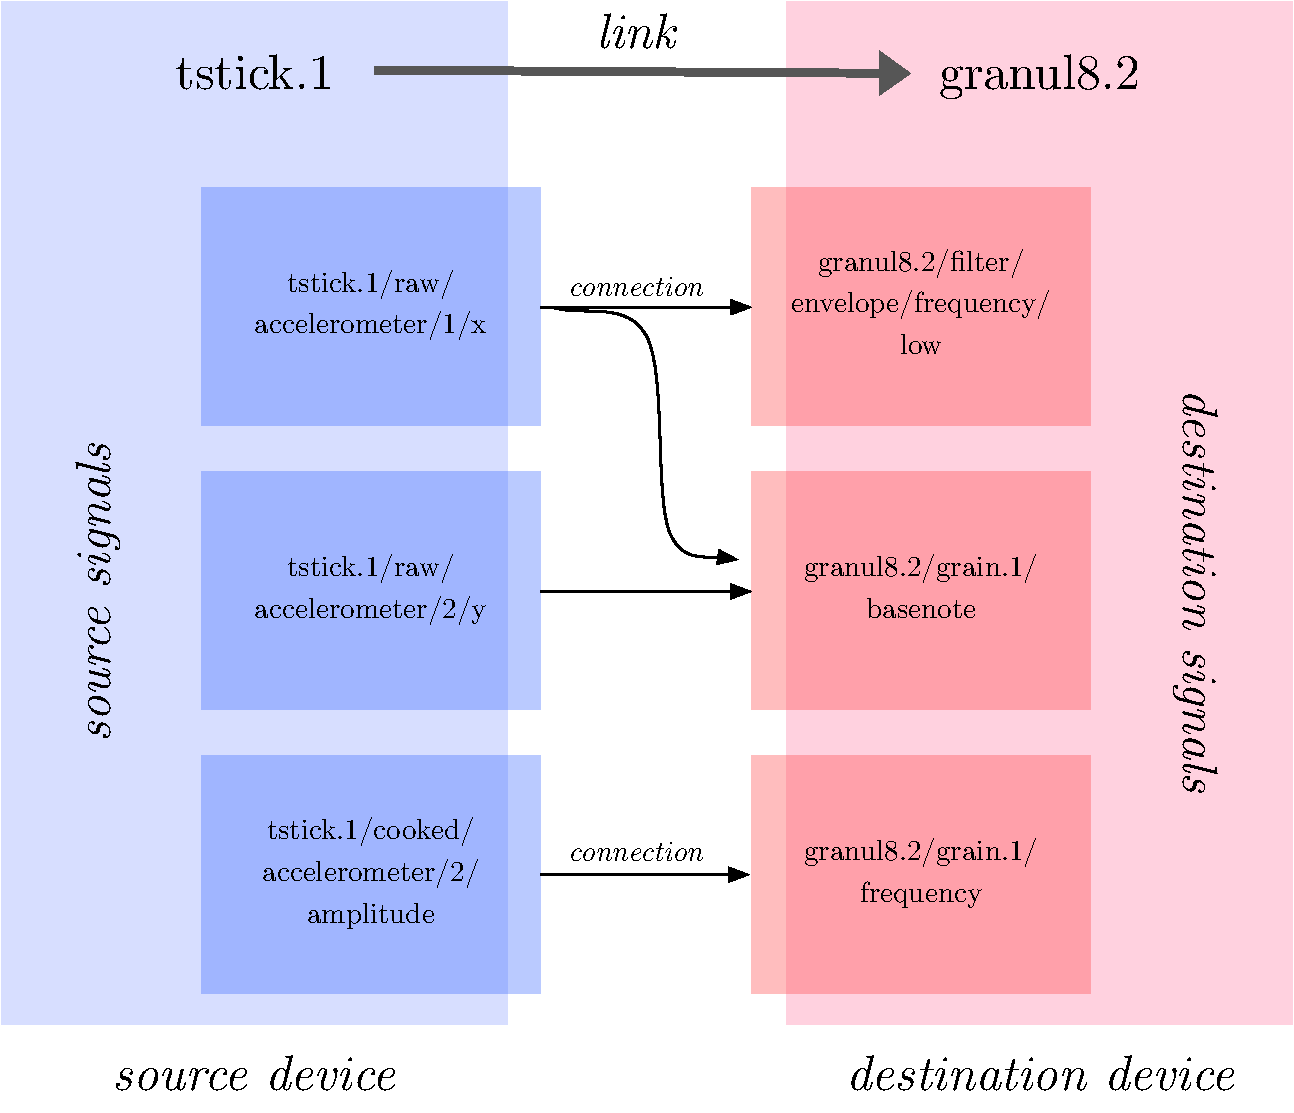
\includegraphics{figures/libmapper_devices}}
\caption{A simple libmapper network}
\label{fig:libmapper_devices}
\end{figure}

Devices and signals can carry a variety of \emph{metadata}. Devices usually list the number of child signals they possess and their location on the network (IP address and port). As previously stated users can tag devices and signals with arbitrary metadata. Connections have a much more specific set of metadata.

%%%%%%%%%%%%%%%%%%%%%%%%%%%%%%%%%%%%%%%%%%%%%%%%%%%%%%%%%%%%%%%%%%%%%%%%%%%%%%%%%%%%%%%%%%%%%%%%%%%%%%%%%%%%%%%%%%%%%%%%%%%%%%%%%%%%%%%%%%%%%%%%%%%%%%%%%%%%%%%%%%%%%%%%%%%%%%%%%%%%%%%%%%%%%%%%%%%%%%%%%%%%%%%%%%%%%%%%%%%%%%%%%%%%%%%%%%%%%%%%%%%%%%%%%%%%%%%%%%
	% section structure_of_libmapper_networks (end)

	\section{Connection Properties} % (fold)
	\label{sec:connection_properties}

Creation of links and connections is mapping from the systems perspective, but libmapper also allows for functional mapping through the modification of connections. This can be accomplished by altering certain properties possessed by every libmapper connection:

\begin{itemize}
	\item\textbf{Expression}: A mathematical equation relating the source ($x$) to destination ($y$) values. An expression of $y = x$ will simply pass through source values, while an expression of $y = 3x + 2$, will apply a linear transformation to the source data (e.g. a value of 1 will be output as 5). libmapper supports a variety of expressions, including exponential functions, trigonometric relations, comparison operators, derivation and integration. 
	\item\textbf{Range}: An array of four numbers containing the user-specified maximum and minimum values for both the source and destination signals.
	\item\textbf{Mode}: The type of connection, this influences the effect of the expression and range properties and can be one of four categories:
	\begin{itemize}
		\item \emph{Linear}: libmapper automatically scales the output such that it fits the destination range, based on the source range. For example, if a certain connection has a source range of $[0, 1]$, and a destination range of $[5, 10]$, libmapper will automatically apply an expression of $y = 5x + 5$, such that the minimum and maximum source values will correspond to the minimum and maximum destination values respectively. A source value that is outside of this source range will result in a destination value that is also outside of the range. In this mode the user cannot directly modify the expression. 
		\item \emph{Calibration}: The same as the linear mode except the source range parameter is ignored. libmapper instead polls the source signal to find the source range directly.
		\item \emph{Bypass}: Source values are sent directly through to the destination signal, as would happen with an expression $y = x$.
		\item \emph{Expression}: The user is able to set the expression to any arbitrary relation.
	\end{itemize}
	\item\textbf{Boundary}: What is to happen to data values when they extend beyond the destination range. There are four options:
	\begin{itemize}
		\item\emph{None}: Values are passed through unchanged.
		\item\emph{Clamp}: Values outside of the boundary are constrained to that value.
		\item\emph{Mute}: No values outside of the boundary are passed to the output.
		\item\emph{Wrap}: Values exceeding the maximum are ``wrapped'' back to the minimum bound and vice versa.
		\item\emph{Fold}: When the signal passes outside of the boundary, the value is inverted back onto the destination range. 
	\end{itemize}
	\item\textbf{Mute}: A true-or-false value muting and un-muting data sent over the connection.
	\item\textbf{Send as instance}: Not all signals on libmapper networks are unique and long lasting, a good example being a keypress on a keyboard. During the keypress, data like aftertouch and release can be sent, making it a bona fide signal. However, musicians constantly create and complete keypress events during performance with keyboard instruments. To maintain every keypress as a unique signal with unique metadata would be tremendously unhelpful for mapping. Also, forcing a user to map every keypress event individually would make live performance impossible.

	To support this, libmapper gives connections the \emph{send as instance} property. Sending data as an instance means that libmapper treats the connected signals as instances of a general class of signals. New instances of a signal class will be treated like previous instances and do not need to be mapped individually.
	\item\textbf{Link scope}: Not a property of connections, but of links. By default links are ``scoped'' to notify destination devices of the creation and destruction of signal instances on linked source devices. For intermediate devices, ones that function as both source and destination, this may not be the desired behavior. If device \url{A} is linked to intermediate device \url{B}, which is in turn linked to device \url{C}, then \url{C} will not be notified of instance events on \url{A} with default link scope settings. The user can modify the scope of link \url{B} $\rightarrow$ \url{C} to include \url{A} if desired.

\end{itemize}

% section connection_properties (end)

%%%%%%%%%%%%%%%%%%%%%%%%%%%%%%%%%%%%%%%%%%%%%%%%%%%%%%%%%%%%%%%%%%%%%%%%%%%%%%%%%%%%%%%%%%%%%%%%%%%%%%%%%%%%%%%%%%%%%%%%%%%%%%%%%%%%%%%%%%%%%%%%%%%%%%%%%%%%%%%%%%%%%%%%%%%%%%%%%%%%%%%%%%%%%%%%%%%%%%%%%%%%%%%%%%%%%%%%%%%%%%%%%%%%%%%%%%%%%%%%%%%%%%%%%%%%%%%%%%
	\section{libmapper Bindings} % (fold)
	\label{sec:libmapper_bindings}

A final crucial libmapper feature is its multi-language \emph{bindings}. The C language is ``low-level'' in that it is very and does not allow for very abstract data structures. This makes it extremely flexible, but difficult and time consuming to use. To make libmapper more friendly for different kinds of developers, ``bindings'' have been created for the higher-level 
Python\footnote{Python Programming Language - Official Website. [Online]. Available: \url{http://www.python.org/}. Accessed July 17, 2013} 
and 
Java\footnote{java.com: Java + You. [Online]. Available: \url{java.com/en}. Accessed July 17, 2013} 
programming languages. libmapper functions are bound to other languages using the 
Simplified Wrapper and Interface Generator (SWIG)\footnote{Simplified Wrapper and Interface Generator. [Online]. Available: \url{http://www.swig.org/}. Accessed July 17, 2013}.
SWIG automatically writes a kind of dictionary that interprets function calls from other languages to the original C. Automatically generated files sit in-between the controlling code and the original library. 

Though concept of ``mapping'' itself is extremely abstract, the libmapper API places it into a concrete context. libmapper is not only means of organizing networks though the creation and destruction of links and connections, it is also a tool for customizing response by its support for modifying connection properties. In this way it can serve both the high-level systems perspective and the low-level functional view of mapping. Though designed for musical devices, the API's loose framework could readily be applied to any type of multimedia system. libmapper is an extremely powerful, flexible tool and requires a user interface that can elegantly deploy its full range of capabilities.

% section libmapper_bindings (end)

%%%%%%%%%%%%%%%%%%%%%%%%%%%%%%%%%%%%%%%%%%%%%%%%%%%%%%%%%%%%%%%%%%%%%%%%%%%%%%%%%%%%%%%%%%%%%%%%%%%%%%%%%%%%%%%%%%%%%%%%%%%%%%%%%%%%%%%%%%%%%%%%%%%%%%%%%%%%%%%%%%%%%%%%%%%%%%%%%%%%%%%%%%%%%%%%%%%%%%%%%%%%%%%%%%%%%%%%%%%%%%%%%%%%%%%%%%%%%%%%%%%%%%%%%%%%%%%%%%
\section{Prior Interfaces for libmapper} % (fold)
\label{sec:prior_interfaces_for_libmapper}

	\subsection{Maxmapper} % (fold)
	\label{sub:maxmapper}

\begin{figure}[h]
	\centering
	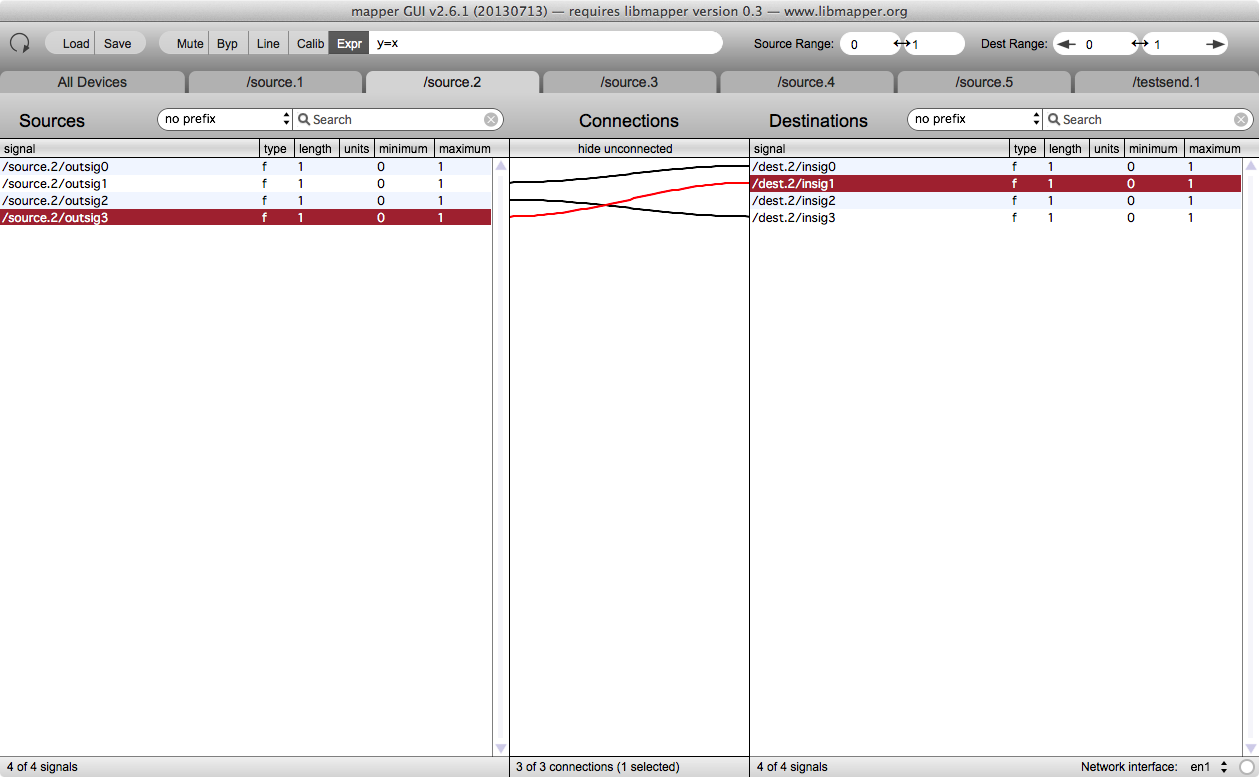
\includegraphics[width=\textwidth]{figures/maxmapper}
	\caption{The Maxmapper interface}
	\label{fig:maxmapper}
\end{figure}

At the beginning of this project the most commonly used GUI for libmapper was a Max/MSP application designed by Joseph Malloch at IDMIL, referred to here as Maxmapper. A list-style interface (see Section \ref{sub:ListView}), Maxmapper allows users to connect signals by dragging between elements on two tables. All source devices are listed in an array of tabs above, clicking on these tabs displays child signals for the device, as well as child signals for all linked devices. The GUI features a top toolbar for saving, loading and editing signal behavior. Maxmapper is extremely functional, and has been used with a wide variety of projects, performances and experiments. To many libmapper users, Maxmapper \emph{is} libmapper.
	
Though Max/MSP works well for creative uses, as well as for prototyping software, it has some well-known limitations that inhibit the functionality of programs like Maxmapper. All Max/MSP standalones must be bundled with a set of necessary objects from Max/MSP itself. This leads to much larger programs, currently Maxmapper occupies nearly 16 times as much computer memory as the MapperGUI standalone.\footnote{22.1 megabytes versus 1.4 megabyes.} The program is also relatively slow to launch, and requires a larger share of computer resources than other implementations. Due to the dependent nature of the code, it is also difficult to maintain and extend Maxmapper, as updates to Max/MSP can cause errors for the program.

The greatest limitation of Maxmapper, and the principal motivation for this project, is the cross-incompatibilty of Max/MSP. The program does not run on Linux systems, and cannot be ported to mobile applications. For the creators of libmapper, this is seen as a fatal flaw. For libmapper to be successful it must be widely adopted, and to dis-include all non-Widows or Macintosh users is unacceptable.
	% subsection maxmapper (end)

	\subsection{Vizmapper} % (fold)
	\label{sub:vizmapper}

\begin{figure}[h]
	\centering
	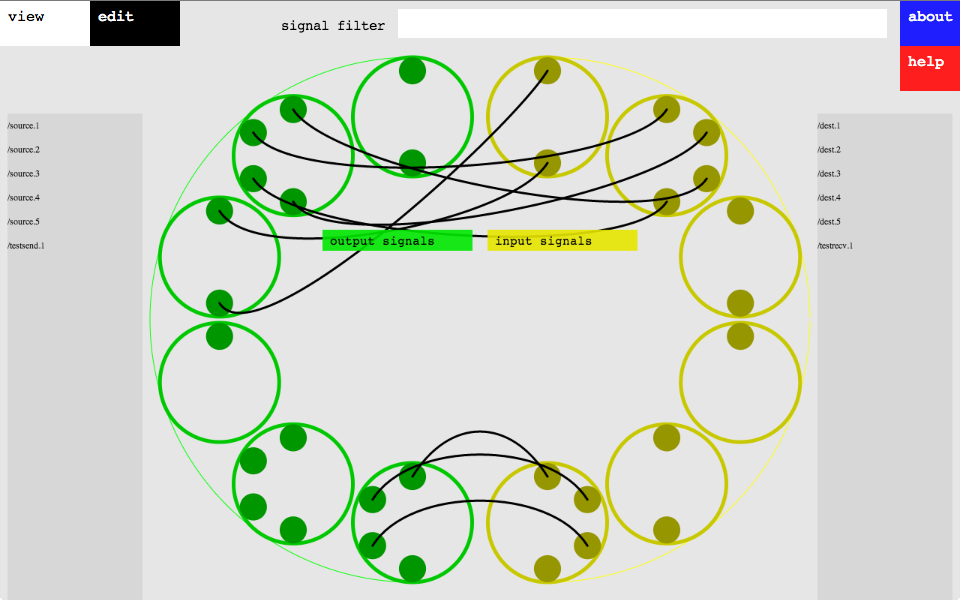
\includegraphics[width=\textwidth]{figures/vizmapper2}
	\caption{The Vizmapper interface}
	\label{fig:vizmapper}
\end{figure}

List-style views for libmapper do not scale well for large and complex networks. To address this need, the Vizmapper provides a novel visualization tool for libmapper networks \cite{vizmapper}. In Vizmapper devices and signals are symbolized by circles distributed about the perimeter of a central screen. Unlike other interfaces, Vizmapper allows the user to zoom in on particular groups of signals, if their names imply some kind of heirarchical structure. For example, the signals \url{tstick.1/raw/accelerometer/1/x} and \url{tstick.1/raw/accelerometer/1/y} are displayed as two different circles within the circle \url{tstick.1/raw/accelerometer/1}. By clicking on this circle the view redraws the left portion of the display to only show signals which are sub-signals of the T-Stick's first accelerometer. 

In this way Vizmapper is capable of displaying all connections on a network simultanously, giving the user a better impression of overall structure. Unfortuantely many functionalities of Maxmapper are not included in Vizmapper. Notably the user can only form connections and links by navigating menus and editing text (as opposed to dragging between nodes). In order to benefit both from the visualization of Vizmapper and the interactibility of Maxmapper, a user would need to run both simultaneously, hence our motivation to integrate approaches. Vizmapper's ``whole network'' visualization is mimiced in the HiveView visualization for MapperGUI, described in Section \ref{sec:alternate_views}.
	
	% subsection vizmapper (end)

	\subsection{Webmapper} % (fold)
	\label{sub:webmapper}
	
\begin{figure}[ht]
	\centering
	%\scalebox{0.42}{
	\includegraphics[width=1\textwidth]%
		{figures/webmapper}
	\caption{The Webmapper interface}
	\label{fig:webmapper}
\end{figure}

Work on this project began with a moderately featured, little used GUI for libmapper known as ``Webmapper.'' Webmapper was created at IDMIL as an attempt to replace the Max/MSP GUI as the result of limitations described in Section \ref{sub:maxmapper}, the principle among which being the cross-platform incompatibility of Max/MSP. It was thought that a browser-based approach would greatly simplify the process of creating cross-compatibility with all major operating systems and even mobile devices. 

Webmapper utilizes the Python bindings for libmapper by registering an administrative monitor to communicate with a libmapper network. The monitor can create and modify connections or links, as well as query the network as to what devices, signals, links and connections are present. The Webmapper code creates a simple HTTP server and attempts to open Google Chrome\footnote{Chrome Browser. [Online]. Available: \url{https://www.google.com/intl/en/chrome/browser/}. Accessed July 17, 2013} on the host computer. If Google Chrome is not present, the user must navigate directly to the server using the web address \url{localhost:50000}. The monitor communicates with the libmapper network and the local server, the browser is able to see messages the monitor ``posts'' to the server (such as `new device') and respond to them appropriately. The browser in turn can send messages to the server (like `connect') that will propagate up to libmapper itself, eventually resulting in a message cascading back down to the browser reflecting the change to the network (such as `new connection'). 

The interface itself is written for a web browser using the scripting language JavaScript\footnote{JavaScript | MDN. [Online]. Available: \url{https://developer.mozilla.org/en-US/docs/Web/JavaScript}. Accessed July 17, 2013} to control web-standard HyperText Markup Language (HTML) elements and Cascading Style Sheets (CSS). The JavaScript code stores four main data structures: devices, links, connections and signals. The code never directly modifies any of this data, and instead waits for messages relayed from libmapper. For example: if a user creates a new link, Webmapper does not add the link directly to the links array but simply sends a message to the network. If it receives back a `new link' message, only then does it add the new link to the array. This is done to ensure that the data structures within Webmapper always reflect what is actually present.

Figure \ref{fig:webmapper} displays the look of the interface before this project began. Users are able to perform all libmapper functions: connecting, linking and modifying connections, but only the simplest of feature sets is included. In order to form a connection the user must click on a source signal, click on a destination signal and then click on a button labeled ``connect.'' Many useful features of Maxmapper, such as column headers, table sorting, drawing connections and search filtering are not present.

	% subsection webmapper (end)

% section prior_interfaces_for_libmapper (end)

%%%%%%%%%%%%%%%%%%%%%%%%%%%%%%%%%%%%%%%%%%%%%%%%%%%%%%%%%%%%%%%%%%%%%%%%%%%%%%%%%%%%%%%%%%%%%%%%%%%%%%%%%%%%%%%%%%%%%%%%%%%%%%%%%%%%%%%%%%%%%%%%%%%%%%%%%%%%%%%%%%%%%%%%%%%%%%%%%%%%%%%%%%%%%%%%%%%%%%%%%%%%%%%%%%%%%%%%%%%%%%%%%%%%%%%%%%%%%%%%%%%%%%%%%%%%%%%%%%
\section{Evaluation of libmapper Variables as Visual Data} % (fold)
\label{sec:evaluation_of_libmapper_variables}

In order to examine different possibilities for visually encoding libmapper data, we have compiled a list variables and their categories as described by \citeN{visual_dimensions}. The list in table \ref{tab:metadata_types} is by no means a complete set, as libmapper may yet expand to include data like device position and users are able to tag devices/signals/links/connections with any extra data they may want.

A fourth data category \emph{boolean} has been added to specify data that only has two values (\emph{true or false}), as it is a common metadata feature. Boolean information is not covered in the Mackinlay paper. Going forward it will be treated more or less like ordinal data.

\begin{longtable}{l l p{4cm} l}
\caption[libmapper metadata types]{libmapper metadata types} \label{tab:metadata_types} \\

	\hline\hline
	\textbf{Devices} & & \\
	\emph{quantitative} & \emph{ordinal} & \emph{nominal}\\
	\hline
	number of inputs & device ordinal & device name\\
		number of outputs \\
	ip address \\
	port \\ [0.7cm]

	\hline\hline
	\textbf{Signals} & & \\
	\emph{quantitative} & \emph{ordinal} & \emph{nominal}\\
	\hline
	length & direction & parent device name\\
	minimum value & & signal name \\
	maximum value & & data type (float, integer, etc.)\\
	sampling rate & & units \\ [0.7cm]

	\hline\hline
	\textbf{Links} & & \\
	\emph{quantitative} & \emph{ordinal} & \emph{nominal}\\
	\hline
	& & link name \\
	& & source device name \\
	& & destination name \\
	& & scope \\ [0.7cm]

	\hline\hline
	\textbf{Connections} & & \\
	\emph{quantitative} & \emph{ordinal} & \emph{nominal} & \emph{boolean}\\
	\hline
	source minimum & instance number & boundary modes & mute\\
	source maximum & & connection mode & send as instance\\
	destination minimum & & destination data type \\
	destination maximum & & mute \\
	& & expression \\
	& & \\
\end{longtable}

% section evaluation_of_libmapper_variables (end)

